\documentclass[a4paper,12pt]{article}
\usepackage{siunitx}
\usepackage[utf8]{inputenc}
\usepackage{amsmath}
\usepackage{xcolor}
\usepackage{graphicx}
\PassOptionsToPackage{hyphens}{url}
\usepackage[citecolor=blue,breaklinks=true]{hyperref}        % Para enlaces en el documento
\usepackage{fancyhdr}
\usepackage{circuitikz}
\usepackage{amssymb}
\usepackage{animate}
\usepackage{float}
\usepackage{multirow}
\usepackage{longtable}
\usepackage{pgfplots}
\pgfplotsset{compat=1.18}
\usetikzlibrary{shapes.symbols}
\usepackage[a4paper, margin=1in]{geometry}
\usepackage{gensymb}
\usepackage{booktabs}
\usepackage{listings}
\usepackage{enumitem}
\usepackage{microtype}      % Micro-tipografía: reduce overfull hbox automáticamente

% Ajuste de la altura del encabezado
\setlength{\headheight}{76.27646pt}
\addtolength{\topmargin}{-34.27646pt}

\lstdefinestyle{mystyle}{
    language=Matlab,
    inputencoding=utf8,
    backgroundcolor=\color{black!5},
    commentstyle=\color{green!60!black},
    keywordstyle=\color{blue},
    numberstyle=\tiny\color{gray},
    stringstyle=\color{purple},
    basicstyle=\footnotesize\ttfamily,
    breaklines=true,
    captionpos=b,
    keepspaces=true,
    numbers=left,
    numbersep=5pt,
    showstringspaces=false,
}
\lstset{style=mystyle}

\setlength{\parindent}{0pt}
\emergencystretch=3em          % Tolerancia extra para evitar overfull hbox residuales

% Crear la portada manualmente
\begin{document}

% Desactivar la numeración de página para la portada
\thispagestyle{empty}

% Colocar las imágenes en las esquinas superiores
\begin{minipage}[t]{0.4\textwidth}
    \raggedright
    
\includegraphics[width=2cm]{image/der.png}
\end{minipage}%
\begin{minipage}[t]{0.5\textwidth}
    \raggedleft
    
\includegraphics[width=2cm]{image/izq.png}
\end{minipage}

\vspace{1cm}

\begin{center}
    \Huge{\textbf{Práctica Complementaria y Obligatoria 11.  Redes Privadas Virtuales (VPN).}} \\
    \vspace{0.5cm}
    \Huge{\textbf{Cuestionario Previo.}} \\
    \vspace{1.5cm}
    \Large{\textbf{Universidad Nacional Autónoma de México.}}\\
    \Large{\textbf{Facultad de Ingeniería.}}\\
    \vspace{1cm}
    \Large{Redes de Datos Seguras.} \\
    \vspace{0.5cm}
    \LARGE{\textbf{Profesora:}}
    \LARGE{\textit{MTRA. MARIA EUGENIA BAUTISTA GONZALEZ.}}\\
    \vspace{0.5cm}
    \Large{\textbf{Grupo:} 02} \\
    \vspace{0.5cm}
    \LARGE{\textbf{Alumno:}}\\
    \Large{320060829} \\
    \vspace{3cm}
    \Large{\textbf{Fecha de Entrega:}}\\
    \vspace{0.5cm}
    \large{{Mayo 08, 2026}}
\end{center}

\newpage

% Configuración del encabezado y pie de página
\pagestyle{fancy}
\fancyhf{}
\fancyhead[L]{
\includegraphics[width=1.5cm]{image/izq.png}}
\fancyhead[R]{
\includegraphics[width=1.5cm]{image/der.png}}
\fancyfoot[C]{\thepage}  % Coloca el número de página en el centro del pie de página

% Línea horizontal en el pie de página
\renewcommand{\footrulewidth}{0.4pt}  % Define el grosor de la línea en el pie de página

% Empezar numeración de páginas desde 1 en la segunda página
\pagenumbering{arabic}
\setcounter{page}{1}

\tableofcontents

\newpage

% ======================================================================
\section{Mencione y describa 3 ejemplos del uso de una VPN.}

Las Redes Privadas Virtuales (VPN, por sus siglas en inglés) han evolucionado desde ser herramientas exclusivas para corporaciones multinacionales hasta convertirse en utilidades indispensables para la ciberseguridad cotidiana. La capacidad de una VPN para cifrar el tráfico y enmascarar la dirección de Protocolo de Internet (IP) permite su aplicación en diversos escenarios, resolviendo problemas de confidencialidad, rentabilidad y control de acceso. A continuación, se describen con exhaustividad tres de los ejemplos de uso más prominentes en el entorno digital actual \cite{aws_vpn, paloalto_vpn_business}.

\textbf{1. Teletrabajo y Acceso Remoto Seguro Corporativo:}
El paradigma laboral contemporáneo ha descentralizado la fuerza de trabajo, obligando a los empleados a operar desde ubicaciones geográficamente dispersas, como hogares, aeropuertos y espacios de trabajo compartido (coworking). En este contexto, conectar un dispositivo directamente a la red corporativa a través de Internet público expone datos empresariales altamente sensibles (como propiedad intelectual, datos financieros y registros de clientes) a interceptaciones maliciosas \cite{trendmicro_vpn}. Las empresas implementan VPN de acceso remoto para mitigar este riesgo. Cuando un empleado remoto inicia su cliente VPN, se establece un túnel cifrado (típicamente utilizando protocolos como IPsec u OpenVPN) entre su dispositivo y el Servidor de Acceso a la Red (NAS) o concentrador VPN de la empresa. Todo el tráfico que fluye a través de este túnel está codificado matemáticamente, garantizando que, incluso si el empleado está utilizando una red Wi-Fi pública e insegura, los atacantes que realicen técnicas de \textit{sniffing} o ataques de intermediario (Man-in-the-Middle) solo percibirán texto cifrado ininteligible. Esto permite al usuario interactuar con la intranet, servidores de archivos internos y bases de datos locales con la misma seguridad lógica que si su equipo estuviera conectado físicamente mediante un cable Ethernet en las oficinas centrales \cite{cloudflare_business}.

\textbf{2. Interconexión Rentable de Sucursales (Site-to-Site):}
Las organizaciones que poseen múltiples oficinas en distintas ciudades o países enfrentan el desafío de mantener una infraestructura de red cohesionada. Históricamente, interconectar estas sucursales requería el arrendamiento de líneas dedicadas físicas o circuitos de Conmutación de Etiquetas Multiprotocolo (MPLS), soluciones que implican altos costos de capital (CapEx) y de operación (OpEx), además de largos tiempos de aprovisionamiento \cite{cisco_vpn_types}. Como alternativa moderna y rentable, las empresas despliegan VPN de sitio a sitio (Site-to-Site VPN). En este escenario, en lugar de instalar software cliente en cada computadora, se instalan pasarelas o enrutadores VPN en el perímetro de cada sucursal. Estos enrutadores establecen túneles cifrados permanentes entre sí a través de la infraestructura pública y económica de Internet \cite{fortinet_site}. Así, la red de área local (LAN) de la sucursal A se integra lógicamente con la LAN de la sucursal B, formando una gran red de área amplia (WAN) virtual. Los usuarios de ambas oficinas pueden compartir servidores, impresoras y sistemas telefónicos de manera transparente, mientras la criptografía subyacente asegura la privacidad de las comunicaciones interempresariales sin la necesidad de costosos enlaces físicos dedicados \cite{ibm_vpn}.

\textbf{3. Evasión de la Censura y Protección de la Identidad en Redes Públicas:}
A nivel individual y de consumidor, las VPN se utilizan prolíficamente para defender los derechos digitales, la privacidad personal y evadir restricciones geográficas. Cuando un usuario se conecta a Internet sin protección, su Proveedor de Servicios de Internet (ISP) y los administradores de las redes locales pueden registrar y auditar su historial de navegación, consultas DNS e interceptar credenciales no cifradas. Además, la dirección IP pública revela la ubicación geográfica aproximada del usuario \cite{kaspersky_vpn}. Al emplear una VPN comercial, el tráfico del usuario se cifra y se redirige a un servidor ubicado en otra región o país. El sitio web de destino no percibe la dirección IP original del usuario, sino la del servidor VPN, proporcionando un manto de anonimato \cite{aws_vpn}. Esto tiene aplicaciones vitales para periodistas y disidentes en regímenes autoritarios, quienes utilizan las VPN para atravesar cortafuegos gubernamentales y acceder a información censurada. De manera paralela, permite a los usuarios sortear bloqueos geográficos impuestos por plataformas de transmisión de video, permitiéndoles acceder a catálogos de contenido globales al aparentar lógicamente que su conexión se origina en la jurisdicción del servidor VPN \cite{nordvpn_uses}.


\newpage
\section{Investigue al menos 5 nombres de proveedores de VPN.}

El ecosistema de proveedores de Redes Privadas Virtuales se ha diversificado enormemente, impulsado por la creciente conciencia sobre la privacidad de los datos y las demandas corporativas de trabajo remoto. A continuación, se presenta un análisis detallado de cinco de los proveedores de VPN comerciales y corporativos más prominentes y confiables del mercado, evaluados bajo métricas de infraestructura, protocolos criptográficos y políticas de retención de datos \cite{top10vpn_2026, xataka_vpn_2026, gizmodo_vpn}.

{
    \renewcommand{\arraystretch}{1.3}
    \begin{longtable}{|p{3cm}|p{3.5cm}|p{3cm}|p{5cm}|}
        \caption{Comparativa de Proveedores de VPN Destacados en el Mercado} \\
        \hline
        \textbf{Proveedor} & \textbf{Sede y Jurisdicción} & \textbf{Protocolos Principales} & \textbf{Característica Distintiva (Insight Técnico)} \\
        \hline
        \endfirsthead
        
        \multicolumn{4}{c}{{\bfseries \tablename\ \thetable{} -- Continuación}} \\
        \hline
        \textbf{Proveedor} & \textbf{Sede y Jurisdicción} & \textbf{Protocolos Principales} & \textbf{Característica Distintiva (Insight Técnico)} \\
        \hline
        \endhead
        
        \hline
        \endfoot
        
        \hline
        \endlastfoot

        \textbf{Proton VPN} & Ginebra, Suiza & WireGuard, OpenVPN, Stealth & Arquitectura \textit{Secure Core}. Enruta el tráfico crítico primero a través de servidores ubicados en búnkeres subterráneos en países respetuosos con la privacidad (fuera de la jurisdicción "Five Eyes") antes de salir al destino final, mitigando ataques de correlación de red \cite{gizmodo_vpn}. \\
        \hline
        \textbf{NordVPN} & Ciudad de Panamá, Panamá & NordLynx, OpenVPN, IKEv2 & Protocolo propietario \textit{NordLynx}, una bifurcación altamente optimizada de WireGuard que incorpora un sistema de doble traducción de direcciones de red (NAT) para asegurar la no persistencia de direcciones IP estáticas en el servidor \cite{nordvpn_uses, xataka_vpn_2026}. \\
        \hline
        \textbf{ExpressVPN} & Islas Vírgenes Británicas & Lightway, OpenVPN, IKEv2/IPsec & Tecnología \textit{TrustedServer}. Todos sus servidores globales operan exclusivamente en memoria volátil (RAM-only), lo que garantiza matemáticamente y arquitectónicamente que ningún dato o registro (\textit{log}) puede sobrevivir a un reinicio del hardware \cite{gizmodo_vpn}. \\
        \hline
        \textbf{Surfshark} & Ámsterdam, Países Bajos & WireGuard, OpenVPN, IKEv2 & Tecnología de enrutamiento \textit{Nexus}. A diferencia de las conexiones tradicionales punto a punto, conecta al usuario a toda una red mallada de servidores simultáneamente, permitiendo la rotación dinámica de IP sin desconexión y ofuscando profundamente el origen del tráfico \cite{gizmodo_vpn}. \\
        \hline
        \textbf{Private Internet Access (PIA)} & Denver, Estados Unidos & WireGuard, OpenVPN, IPsec & Altamente apreciado por administradores de sistemas debido a su código parcialmente abierto (\textit{open-source}) y su inmensa infraestructura (más de 35,000 servidores). Permite personalización granular a nivel de criptografía (intercambio dinámico entre AES-128 y AES-256) \cite{gizmodo_vpn}. \\
    \end{longtable}
}

Es pertinente mencionar que, en ámbitos puramente empresariales, las organizaciones tienden a depender de infraestructuras VPN suministradas por fabricantes de *hardware* y *software* de seguridad de borde, tales como \textbf{Cisco (AnyConnect)}, \textbf{Palo Alto Networks (GlobalProtect)}, y \textbf{Fortinet (FortiClient)} \cite{cisco_vpn_types, checkpoint_vpn_enterprise}. Estos proveedores integran las capacidades VPN dentro de marcos holísticos de Seguridad de Confianza Cero (Zero Trust Network Access, ZTNA) y plataformas SASE (Secure Access Service Edge), permitiendo a los departamentos de TI aplicar políticas de acceso basadas en la identidad y en la postura de seguridad del dispositivo \cite{zscaler_vpn}.


\newpage
\section{Dibuje y describa un diagrama de cómo funciona un servicio de VPN.}

El funcionamiento de un servicio VPN es una orquestación sofisticada de algoritmos criptográficos, manipulación de tablas de enrutamiento y tunelización de red. A continuación, se presenta un diagrama esquemático que ilustra el flujo de datos desde el dispositivo del usuario final hasta el servidor de destino a través de la infraestructura pública, seguido de una disección técnica del proceso.

\begin{figure}[H]
    \centering
    \begin{tikzpicture}[>=stealth, thick]
        % Colores
        \definecolor{userblue}{RGB}{70, 130, 180}
        \definecolor{vpnred}{RGB}{220, 20, 60}
        \definecolor{internetgray}{RGB}{200, 200, 200}
        \definecolor{destgreen}{RGB}{34, 139, 34}

        % Nodos
        \node[draw, rounded corners, fill=userblue!20, minimum width=2.5cm, minimum height=1.5cm, align=center] (client) at (0,0) {\textbf{Dispositivo}\\\textbf{Cliente}\\(Con App VPN)};
        
        \node[draw, cloud, fill=internetgray!30, cloud puffs=12, cloud puff arc=120, aspect=2, minimum width=4cm, minimum height=2cm, align=center] (internet) at (5,0) {\textbf{Internet}\\\textbf{Público}\\(Túnel Cifrado)};
        
        \node[draw, rounded corners, fill=vpnred!20, minimum width=2.5cm, minimum height=1.5cm, align=center] (vpnserver) at (10,0) {\textbf{Servidor}\\\textbf{VPN}\\(Descifra y Enruta)};
        
        \node[draw, rounded corners, fill=destgreen!20, minimum width=2.5cm, minimum height=1.5cm, align=center] (destination) at (15,0) {\textbf{Servidor}\\\textbf{Destino}\\(Sitio Web/Red)};

        % Conexiones
        \draw[->, color=red, line width=1.5pt] (client) -- node[above] {\small Cifrado} (internet);
        \draw[->, color=red, line width=1.5pt] (internet) -- node[above] {\small Encapsulado} (vpnserver);
        \draw[->, color=black, line width=1pt] (vpnserver) -- node[above] {\small Texto Claro} (destination);
        
        % Retorno
        \draw[<-, color=black, line width=1pt] (vpnserver.south east) ++(0,-0.5) -- node[below] {\small Respuesta} (destination.south west);
        \draw[<-, color=red, line width=1.5pt] (internet.south) ++(3.5,-0.5) -- node[below] {\small Cifrado} (vpnserver.south west);
        \draw[<-, color=red, line width=1.5pt] (client.south east) ++(0,-0.5) -- node[below] {\small Tránsito Seguro} (internet.south) ++(-1.5,-0.5);

        % Leyenda de cifrado
        \node[align=left, text width=5cm] at (5,-2.5) {\textit{\textcolor{red}{Línea Roja:} Datos cifrados e ilegibles para el ISP.}};
        \node[align=left, text width=5cm] at (11.5,-2.5) {\textit{Línea Negra: Datos estándar en Internet.}};

    \end{tikzpicture}
    \caption{Diagrama del Flujo Lógico y Tunelización Cifrada en una VPN.}
\end{figure}

\textbf{Descripción del Proceso de Tunelización:}

El mecanismo de tunelización no implica un conducto físico, sino una técnica de encapsulación lógica a nivel de paquetes de red \cite{ibm_vpn_steps}. La transmisión se articula a través de las siguientes fases críticas \cite{nordvpn_how_it_works, ibm_vpn_steps, fortinet_vpn_how}:

1. \textbf{Inicialización e Interfaz Virtual:} Al iniciar el cliente VPN, el software integra un adaptador de red virtual en el sistema operativo (típicamente empleando interfaces \texttt{TUN/TAP}). El sistema operativo modifica sus tablas de enrutamiento para forzar que todo el tráfico saliente abandone el equipo exclusivamente a través de esta interfaz virtual.

2. \textbf{Handshake (Negociación Criptográfica):} Antes del intercambio de carga útil (datos), el cliente y el servidor VPN ejecutan un \textit{handshake} o saludo. Utilizando criptografía asimétrica (como RSA o Curva Elíptica) y protocolos de intercambio de claves como \textit{Diffie-Hellman}, ambas entidades se autentican mutuamente y acuerdan una clave simétrica efímera de sesión. Esta clave garantizará que solo ellos puedan codificar y decodificar el tráfico subsecuente.

3. \textbf{Cifrado y Encapsulación:} Cuando el usuario intenta acceder a un recurso en la red, el cliente VPN intercepta el paquete de datos original (que contiene el mensaje y la IP de destino final). El cliente cifra todo este paquete utilizando algoritmos robustos como AES-256. Posteriormente, envuelve o "encapsula" este paquete ilegible dentro de un nuevo paquete IP exterior, cuya única dirección de destino es la IP del Servidor VPN.

4. \textbf{Tránsito a través de Infraestructura No Confiable:} El paquete encapsulado viaja a través del enrutador local y el Proveedor de Servicios de Internet (ISP). El ISP únicamente observa un flujo de datos ininteligible dirigido hacia un servidor VPN; es incapaz de inspeccionar el contenido del paquete original o conocer el verdadero destino final en Internet.

5. \textbf{Descifrado y Enmascaramiento de IP (NAT):} Al recibir el paquete, el Servidor VPN descarta la cabecera exterior y utiliza la clave de sesión simétrica para descifrar el interior. Se revela la solicitud original del usuario. El servidor VPN actúa como un \textit{proxy} o intermediario: altera la dirección IP de origen del paquete (sustituyendo la IP real del usuario por la IP del propio servidor) y reenvía la petición al destino final.

6. \textbf{Retorno de Datos:} El Servidor Destino procesa la solicitud y envía la respuesta de vuelta al Servidor VPN (creyendo que este es el originador). El Servidor VPN cifra instantáneamente esta respuesta y la envía a través del túnel seguro de vuelta al cliente, completando el ciclo de comunicación confidencial.


\newpage
\section{¿Qué características de seguridad provee una VPN?}

La solidez y eficacia de una Red Privada Virtual se fundamentan en su capacidad para satisfacer los postulados del modelo más crítico de la ciberseguridad, conocido como la \textbf{Tríada CIA} (Confidencialidad, Integridad y Disponibilidad), complementada con la autenticación rigurosa \cite{checkpoint_vpn, netwrix_cia}. Las características de seguridad intrínsecas que provee una VPN para cumplir este modelo son:

\textbf{1. Confidencialidad a través de Cifrado Fuerte:}
La característica más destacada de una VPN es la confidencialidad, la cual garantiza que la información en tránsito sea ininteligible para actores no autorizados \cite{aws_vpn}. Esto se logra implementando algoritmos de cifrado simétrico de grado militar, predominantemente el \textit{Advanced Encryption Standard} (AES) con claves de 256 bits, o algoritmos más modernos como ChaCha20 (utilizado por el protocolo WireGuard) \cite{ibm_vpn}. La entropía de una clave de 256 bits es tan vasta que un ataque de fuerza bruta requeriría supercomputadoras operando durante miles de millones de años para descifrar un solo paquete de datos \cite{kaspersky_vpn}. Esto previene eficazmente la interceptación de datos en redes Wi-Fi comprometidas y neutraliza el espionaje corporativo o gubernamental.

\textbf{2. Integridad de Datos mediante Funciones Hash:}
La integridad asegura que los paquetes de datos no sean alterados, inyectados con código malicioso (malware) ni corrompidos durante su trayecto a través de Internet \cite{cisco_vpn_ccna}. Las VPN implementan este control utilizando funciones de resumen criptográfico (Hash) junto con Códigos de Autenticación de Mensajes Basados en Hash (HMAC), como HMAC SHA-256 o SHA-384 \cite{protonvpn_protocols}. Al momento de emitir un paquete, el cliente VPN genera una "firma matemática" única del contenido. Al recibirlo, el servidor VPN ejecuta la misma ecuación; si el resultado difiere por un solo bit, la red deduce que el paquete fue manipulado en el trayecto y lo descarta inmediatamente, abortando potenciales ataques de modificación activa \cite{netwrix_cia}.

\textbf{3. Autenticación Mutua y Gestión de Identidades:}
Una VPN no solo protege la carga útil, sino que restringe el acceso al túnel en sí. La infraestructura implementa autenticación rigurosa para verificar la identidad de ambas partes (el cliente remoto y la pasarela VPN). Esto se gestiona mediante Infraestructuras de Clave Pública (PKI), certificados digitales (X.509) o claves precompartidas (PSK) negociadas durante el establecimiento del protocolo IKEv2 o TLS \cite{cisco_vpn_technologies}. En entornos corporativos avanzados, esta característica se refuerza con Autenticación Multifactor (MFA) y posturas de acceso de confianza cero (ZTNA), mitigando el riesgo de credenciales comprometidas o intentos de suplantación de identidad \cite{zscaler_vpn, fortinet_site}.

\textbf{4. Enmascaramiento y Evasión (Ofuscación):}
Para prevenir ataques dirigidos y mantener el anonimato, las VPN proveen enmascaramiento de la dirección IP. Al actuar como intermediario en las solicitudes DNS y web, la VPN asume el perfil público del cliente, protegiendo al dispositivo de origen frente a escaneos de puertos perimetrales y ataques de Denegación de Servicio (DoS) \cite{aws_vpn, ibm_vpn}. Además, las VPN modernas incluyen características de protección contra fugas de DNS y WebRTC, junto con un \textit{Kill Switch} automático (Interruptor de corte) que bloquea instantáneamente el tráfico de red de la máquina a nivel de sistema operativo si el túnel cifrado sufre una interrupción accidental, evitando la exposición inadvertida de datos en claro \cite{gizmodo_vpn}.


\newpage
\section{Mencione y describa los distintos tipos de VPN que existen.}

La arquitectura de las redes virtuales no es monolítica; se ha ramificado para adaptarse a diversas topologías de red, casos de uso empresarial y requerimientos de usuarios finales. Las normativas y documentaciones de fabricantes como Cisco y Palo Alto Networks categorizan a las VPN en varios tipos principales basados en cómo establecen las conexiones entre los nodos \cite{paloalto_types, cisco_vpn_types}.

\textbf{1. VPN de Acceso Remoto (Remote Access VPN / Client-to-Site):}
Esta es la arquitectura dominante tanto para el consumidor final como para el teletrabajo empresarial \cite{fortinet_remote}. Permite que un usuario individual, que se encuentra fuera del perímetro físico de la organización, se conecte de forma segura a una red privada alojada centralmente \cite{aws_vpn, paloalto_types}. Requiere la instalación de un software cliente o agente (como Cisco Secure Client o OpenVPN Connect) en el dispositivo del usuario (computadora portátil, tableta o teléfono inteligente). Al establecer la conexión, el dispositivo remoto adquiere una dirección IP virtual dentro del rango de la red local (LAN) de la empresa, lo que le permite acceder a recursos corporativos y servidores de aplicaciones a través de Internet como si estuviera interconectado localmente \cite{cloudflare_business}. 

\textbf{2. VPN de Sitio a Sitio (Site-to-Site VPN / Router-to-Router):}
Las VPN de sitio a sitio están diseñadas para conectar redes enteras en lugar de usuarios individuales. Su propósito fundamental es extender la red corporativa entre la sede central y múltiples sucursales geográficamente distantes sin incurrir en el costo de líneas privadas dedicadas \cite{cisco_vpn_types, paloalto_site}. En este esquema, el túnel cifrado no se origina en un dispositivo final, sino que se establece entre dos pasarelas de seguridad (Firewalls o Routers VPN) ubicadas en los perímetros de cada red. Los dispositivos dentro de estas oficinas no requieren software cliente y a menudo desconocen la existencia de la VPN; simplemente envían tráfico que es transparentemente interceptado, cifrado, enrutado y descifrado por las pasarelas. Se subdividen comúnmente en \textbf{Intranets} (conectando sucursales de la misma empresa) y \textbf{Extranets} (conectando redes de diferentes corporaciones para colaborar con proveedores o socios comerciales de manera controlada) \cite{cisco_vpn_types}. Esta arquitectura depende casi exclusivamente del protocolo IPsec operando en la capa de red \cite{checkpoint_ipsec}.

\textbf{3. VPN SSL (Clientless VPN):}
Una variante del acceso remoto, la VPN SSL (basada en el protocolo Secure Sockets Layer o su sucesor moderno TLS) opera en la capa de aplicación del modelo OSI en lugar de la capa de red \cite{checkpoint_ssl, paloalto_ipsec_vs_ssl}. Su principal diferenciador, a menudo denominado enfoque "sin cliente", es que no requiere la instalación de software especializado en el equipo del usuario \cite{aws_vpn}. El acceso se obtiene exclusivamente a través de un navegador web estándar mediante HTTPS, conectándose a un portal corporativo centralizado. Una VPN SSL otorga un control extremadamente granular: en lugar de proporcionar al usuario acceso a toda la subred de la empresa, el administrador de TI puede restringir el acceso del usuario únicamente a aplicaciones web corporativas específicas \cite{paloalto_ipsec_vs_ssl}. Esta arquitectura minimiza severamente la superficie de ataque y es ideal para proporcionar acceso seguro a contratistas de terceros o empleados que utilizan equipos no gestionados por la empresa (política BYOD - \textit{Bring Your Own Device}).

\textbf{4. VPN Móvil (Mobile VPN):}
A diferencia de las VPN estáticas que asumen una conexión de red ininterrumpida, una VPN móvil está diseñada con alta tolerancia a la intermitencia \cite{cisco_mobile_vpn}. Se utiliza en entornos donde los dispositivos transitan constantemente entre diferentes puntos de acceso a redes, por ejemplo, cambiando de una conexión Wi-Fi inestable a una red celular de banda ancha (LTE/5G). Mientras que una VPN tradicional colapsaría y requeriría una renegociación manual completa del túnel criptográfico al perder su IP pública original, la VPN móvil persiste lógicamente, manteniendo las aplicaciones y el túnel activos en segundo plano hasta que la conectividad física se restaura \cite{cisco_mobile_vpn}. Esto es indispensable para flujos de trabajo críticos de personal de primeros auxilios (policías, paramédicos) o trabajadores de logística móvil en campo.


\newpage
\section{¿Para qué se usa el comando apt-get install pptpd o apt install pptpd?}

En el ecosistema de los sistemas operativos basados en el núcleo de Linux, específicamente en la genealogía de la distribución Debian (como Ubuntu o Linux Mint), la instalación de infraestructuras de red, como un servidor VPN, recae en la administración inteligente de paquetes de software de código abierto.

El comando \texttt{sudo apt-get install pptpd} (o su contraparte moderna, \texttt{sudo apt install pptpd}) tiene un propósito sumamente específico: **indica a la herramienta de gestión de paquetes del sistema operativo que localice, descargue, resuelva las dependencias e instale de forma completamente automatizada el software "pptpd" para convertir a ese servidor Linux en un nodo de red privada virtual** \cite{digitalocean_pptp, geekland_pptp}.

\textbf{El Demonio PPTP (\texttt{pptpd}):}
El acrónimo \texttt{pptpd} hace referencia al \textit{Point-to-Point Tunneling Protocol Daemon}. Se trata de un servicio que se ejecuta en segundo plano en el servidor y que implementa el protocolo de túnel punto a punto (PPTP), desarrollado originalmente por un consorcio liderado por Microsoft en 1999 \cite{ticarte_pptp}. Al instalar este paquete, el servidor adquiere la capacidad de escuchar peticiones de red entrantes en el puerto TCP 1723 y el protocolo GRE (Generic Routing Encapsulation) número 47 \cite{ticarte_pptp, digitalocean_pptp}. Posteriormente, el administrador debe alterar los archivos lógicos de configuración (como \texttt{/etc/pptpd.conf} para asignar el rango de direcciones IP y \texttt{/etc/ppp/chap-secrets} para gestionar los usuarios y contraseñas de la VPN) para completar la infraestructura \cite{digitalocean_pptp, time4vps_pptp}. 

*Nota Crítica de Seguridad:* En la literatura técnica actual de redes seguras, el uso de PPTP está categóricamente desaconsejado para entornos de producción corporativos o información confidencial. Su protocolo de autenticación subyacente (MS-CHAPv2) y el algoritmo de cifrado RC4 de 128 bits son altamente vulnerables y han sido criptográficamente comprometidos, permitiendo que atacantes descifren la carga útil mediante ataques de intercepción \cite{protonvpn_protocols, ticarte_pptp}.

\textbf{Diferencia Arquitectónica entre \texttt{apt-get} y \texttt{apt}:}
Para entender las variantes del comando, es indispensable contextualizar la infraestructura de gestión de paquetes de Debian, conocida como \textit{Advanced Package Tool} (APT). Las herramientas de APT interactúan con el núcleo del sistema (\texttt{dpkg}) pero incorporan inteligencia para buscar dependencias (por ejemplo, al instalar \texttt{pptpd}, APT deducirá y descargará automáticamente paquetes requeridos como \texttt{bcrelay} o \texttt{ppp} sin intervención manual) \cite{aws_apt, cirelramos_pptp}.

\begin{itemize}
    \item \textbf{\texttt{apt-get}:} Es la herramienta clásica, de bajo nivel, introducida en 1998. Está diseñada por naturaleza para ser estricta, estable y predecible. Carece de interfaces visuales sofisticadas. El consenso técnico dicta que \texttt{apt-get} es la única variante que debe usarse dentro de \textit{scripts} de automatización de servidores (Bash scripting), debido a que garantiza compatibilidad retroactiva absoluta y sus salidas no alteran su formato, evitando errores en la automatización \cite{aws_apt, askubuntu_apt}.
    \item \textbf{\texttt{apt}:} Introducido más recientemente (con Debian 8 en 2014), es un subconjunto consolidado de alto nivel diseñado para el uso interactivo del administrador humano. Combina las funciones históricas dispersas en \texttt{apt-get} (para instalación) y \texttt{apt-cache} (para búsquedas de paquetes) en un solo comando amigable \cite{aws_apt}. \texttt{apt} provee retroalimentación visual amigable, como barras de progreso dinámicas, coloreado de sintaxis, e información inmediata sobre paquetes residuales que pueden ser eliminados \cite{aws_apt}.
\end{itemize}

En resumen, invocar este comando inicia la arquitectura base de un servidor VPN legacy en Linux, siendo \texttt{apt} preferido por administradores manuales y \texttt{apt-get} imperativo para rutinas de automatización e infraestructura como código (IaC).


\newpage
\section{Investigue qué es el editor nano y cuáles son sus comandos principales.}

La administración de servidores en arquitecturas de red seguras, como las VPN operadas bajo infraestructuras GNU/Linux, raramente cuenta con Interfaces Gráficas de Usuario (GUI). Las configuraciones de seguridad e integraciones de enrutamiento se realizan íntegramente a través de conexiones remotas encriptadas de línea de comandos mediante Secure Shell (SSH). En este hábitat estricto, la modificación de archivos de texto plano, *scripts* de Bash y parámetros de configuración requiere de procesadores de texto basados en la terminal. En esta categoría reina \textbf{GNU Nano} \cite{arsys_nano, librebyte_nano}.

\textbf{¿Qué es GNU Nano?}

GNU Nano (generalmente referido simplemente como `nano`) es un editor de texto de terminal ligero, de código abierto y no modal, integrado nativamente en casi la totalidad de las distribuciones Linux y Unix contemporáneas \cite{nano_editor_official, arsys_nano}. Originalmente creado en 1999 como un clon libre y mejorado del editor \textit{Pico} (utilizado en el cliente de correo Pine), Nano fue concebido con una filosofía de diseño enfocada radicalmente en la accesibilidad y la intuición del usuario \cite{ubuntu_community_nano}. 

La principal barrera de entrada en la administración de sistemas ha sido históricamente la pronunciada curva de aprendizaje de los editores modales legados, como \texttt{vi} o \texttt{Vim}, que requieren transiciones complejas entre "modos de comando" y "modos de inserción". Nano, por el contrario, despliega una interfaz directa donde las teclas introducen caracteres inmediatamente en el búfer, y exhibe en tiempo real en las dos últimas líneas de la consola un submenú visible (la barra de estado inferior) con los atajos de teclado primordiales de navegación y guardado \cite{librebyte_nano, arsys_nano}. 

A pesar de su aparente simplicidad, Nano es sumamente robusto para ingenieros. Soporta coloreado de sintaxis múltiple (para lenguajes como C, PHP, Bash y HTML), retroceso ilimitado (undo/redo), numeración de líneas, edición asimétrica de múltiples búferes simultáneamente e integración de búsquedas mediante expresiones regulares avanzadas, a menudo parametrizadas mediante su archivo de configuración interno \texttt{.nanorc} \cite{librebyte_nano, nano_editor_official}.

\textbf{Comandos Principales y Atajos de Teclado (Shortcuts)}

En la nomenclatura del ecosistema Nano, las directivas de control estructural se invocan combinando la tecla Control (\texttt{Ctrl}, representada en la interfaz en pantalla mediante el símbolo de intercalación \texttt{\^}) o la tecla Meta (habitualmente la tecla \texttt{Alt} o \texttt{Esc}, representada como \texttt{M-}) y un comando alfabético. A continuación se compendian los atajos fundamentales para el despliegue y modificación de configuraciones de red \cite{librebyte_nano, nano_editor_official, arsys_nano}:

\begin{table}[H]
    \centering
    \renewcommand{\arraystretch}{1.3}
    \caption{Referencia de Comandos Estructurales de GNU Nano}
    \vspace{0.2cm}
    \begin{tabular}{|p{3.5cm}|p{2cm}|p{9cm}|}
        \hline
        \textbf{Acción Operativa} & \textbf{Atajo} & \textbf{Descripción Técnica del Comando} \\
        \hline
        \textbf{Guardar (\textit{Write Out})} & \texttt{Ctrl + O} & Fuerza la escritura del búfer temporal de datos hacia el archivo físico en el sistema de almacenamiento. Solicita confirmación explícita del nombre del archivo antes de inyectar las alteraciones \cite{librebyte_nano, arsys_nano}. \\
        \hline
        \textbf{Salir (\textit{Exit})} & \texttt{Ctrl + X} & Termina la ejecución del binario nano y cierra el editor. Si el búfer ha detectado cambios no guardados, interrumpirá la salida solicitando confirmación al administrador para preservar o purgar las alteraciones \cite{nano_editor_official}. \\
        \hline
        \textbf{Buscar (\textit{Where Is})} & \texttt{Ctrl + W} & Invoca un motor de búsqueda interactiva en el búfer. Permite localizar secuencias textuales simples o evaluar expresiones regulares estructuradas si se combina con Meta-R \cite{librebyte_nano}. \\
        \hline
        \textbf{Cortar (\textit{Cut Text})} & \texttt{Ctrl + K} & Suprime por completo la línea de texto actual donde reside el cursor y la exporta al búfer de corte transitorio (equivalente interno de un portapapeles) \cite{librebyte_nano}. \\
        \hline
        \textbf{Pegar (\textit{Uncut Text})} & \texttt{Ctrl + U} & Importa e imprime en la posición actual del cursor el último fragmento de código preservado en el búfer de corte \cite{nano_editor_official}. \\
        \hline
        \textbf{Información Geográfica} & \texttt{Ctrl + C} & Inyecta un sondeo en tiempo real que imprime en la barra de estado las coordenadas cartesianas exactas del cursor (Línea, Columna, y progreso porcentual del documento) \cite{arsys_nano, nano_editor_official}. \\
        \hline
        \textbf{Deshacer (\textit{Undo})} & \texttt{Alt + U} & Revierte la última inserción de texto o comando destructivo, protegiendo las alteraciones accidentales del archivo \cite{nano_editor_official}. \\
        \hline
    \end{tabular}
\end{table}


\newpage
\section{¿Para que se usa el comando ipconfig en Windows?}

En las arquitecturas locales de clientes Windows, el proceso de diagnóstico y análisis forense de anomalías de conectividad (particularmente durante fallos en la tunelización de VPNs o resoluciones anómalas de dominios corporativos) se apoya en utilitarios integrados ejecutados desde el Símbolo del Sistema (\texttt{cmd.exe}) o \textit{PowerShell}. El ejecutable central para la inspección y manipulación de la pila TCP/IP es \textbf{\texttt{ipconfig}} (Configuración del Protocolo de Internet) \cite{ms_learn_ipconfig, ionos_ipconfig}.

El comando \texttt{ipconfig} es una utilidad de línea de comandos de las interfaces Win32 diseñada para revelar todas las configuraciones actuales del protocolo TCP/IP de un host y forzar la sincronización o regeneración de los parámetros asignados dinámicamente mediante el Protocolo de Configuración Dinámica de Host (DHCP) y el Sistema de Nombres de Dominio (DNS) \cite{ms_learn_ipconfig}. 

Cuando el analista invoca la directriz puramente como \texttt{ipconfig} sin parámetros adicionales, el motor sondea las interfaces y devuelve un sumario conciso. Este reporte básico lista las direcciones lógicas activas (tanto IPv4 como IPv6), la máscara de subred, y la dirección de la puerta de enlace predeterminada (\textit{Default Gateway}) de todos los adaptadores físicos de red (Ethernet y Wi-Fi) y de los adaptadores lógicos virtuales (como las interfaces creadas por los clientes VPN) instalados en el sistema operativo \cite{ms_learn_ipconfig, ionos_ipconfig}. 

Sin embargo, el verdadero poder operativo de \texttt{ipconfig} reside en el uso de parámetros condicionales (indicados mediante el símbolo \texttt{/}), los cuales dotan a la herramienta de capacidades ejecutivas de mitigación y reinicio. Los parámetros más críticos son \cite{ms_learn_ipconfig, ms_learn_ipconfig_renew}:

\begin{itemize}
    \item \textbf{\texttt{ipconfig /all}:} 
    Genera un informe exhaustivo de las propiedades de red. A diferencia de la ejecución básica, esta invocación detalla la Dirección Física subyacente (Dirección MAC), si la concesión de red fue provista manualmente o mediante un protocolo automático (DHCP Enabled), y especifica las ventanas temporales precisas del ciclo de vida del arrendamiento IP (Lease Obtained y Lease Expires). Asimismo, divulga el listado ordenado de todos los servidores DNS asignados, lo cual es vital para auditar vulnerabilidades o fugas de DNS en túneles VPN.

    \item \textbf{\texttt{ipconfig /release}:} 
    Es un comando destructivo deliberado. Al invocarlo, Windows transmite un paquete del tipo \texttt{DHCPRELEASE} al servidor controlador, notificándole que el host renuncia inmediatamente a su arrendamiento de dirección IP vigente \cite{ms_learn_ipconfig_renew}. El adaptador de red seleccionado (o todos, por defecto) interrumpe su conectividad, vaciando sus valores de red a nivel de sistema. Es el primer paso en la mitigación de conflictos de solapamiento o de asignaciones defectuosas en subredes congestionadas.

    \item \textbf{\texttt{ipconfig /renew}:} 
    Consecuencia directa de un comando de liberación (release), este parámetro reactiva al cliente DHCP del sistema operativo, forzándolo a iniciar una fase completa de descubrimiento y renegociación con los servidores locales (proceso DORA: Discover, Offer, Request, Acknowledge) para solicitar la provisión de una nueva configuración y dirección IP \cite{ms_learn_ipconfig_renew}. Restablece la comunicación a nivel de capa de red en entornos caóticos.

    \item \textbf{\texttt{ipconfig /flushdns}:} 
    La mitigación de errores de DNS es, con frecuencia, el escenario más elusivo en las transiciones de acceso remoto VPN \cite{ms_learn_ipconfig_renew}. Windows preserva un almacenamiento dinámico o caché de resoluciones locales de dominios (Client Resolver Cache) para agilizar las reconexiones. Sin embargo, cuando se altera la infraestructura o un servidor interno cambia súbitamente, el caché retiene localizaciones residuales incorrectas (\textit{negative cache entries}). \texttt{/flushdns} destruye forzosamente esta memoria temporal y la purga por completo \cite{ms_learn_ipconfig}. Esto obliga al navegador y a las herramientas de red a volver a someter sus interrogaciones desde cero contra los servidores DNS corporativos provistos por el túnel seguro de la VPN, rectificando el acceso asimétrico a recursos web.
\end{itemize}


\newpage
\begin{thebibliography}{99}
    
    % Pregunta 1: Ejemplos de uso (AWS, Palo Alto, Kaspersky, Cloudflare)
    \bibitem{aws_vpn} 
    Amazon Web Services (AWS). (2026). \textit{¿Qué es una VPN? Ventajas, tipos y arquitectura}. Recuperado de \url{https://aws.amazon.com/es/what-is/vpn/}

    \bibitem{paloalto_vpn_business} 
    Palo Alto Networks. (2026). \textit{¿Qué es una VPN empresarial? Conozca sus usos y limitaciones}. Recuperado de \url{https://www.paloaltonetworks.es/cyberpedia/what-is-a-business-vpn-understand-its-uses-and-limitations}

    \bibitem{trendmicro_vpn} 
    Trend Micro. (2026). \textit{¿Qué es la VPN Protection?}. Recuperado de \url{https://www.trendmicro.com/es_es/what-is/vpn-protection.html}
    
    \bibitem{kaspersky_vpn} 
    Kaspersky. (2026). \textit{¿Qué es una VPN? Cómo funciona, tipos y beneficios}. Recuperado de \url{https://latam.kaspersky.com/resource-center/definitions/what-is-a-vpn}

    \bibitem{nordvpn_uses} 
    NordVPN. (2026). \textit{¿Para qué usan una VPN la mayoría de los usuarios?}. Recuperado de \url{https://nordvpn.com/es/blog/cosas-sabias-podias-hacer-vpn/}

    % Pregunta 2: Proveedores y Análisis (Top10VPN, Gizmodo, Xataka)
    \bibitem{top10vpn_2026} 
    Top10VPN. (2026). \textit{Recomendaciones por propósito y dispositivo: Evaluaciones VPN}. Recuperado de \url{https://www.top10vpn.com/es/mejor-vpn/}

    \bibitem{gizmodo_vpn} 
    Gizmodo. (2026). \textit{Las mejores VPN del mercado: Análisis de privacidad y velocidad}. Recuperado de \url{https://es.gizmodo.com/vpn}

    \bibitem{xataka_vpn_2026} 
    Xataka Basics. (2026). \textit{Mejores VPN 2026: guía con los mejores servicios para proteger tu privacidad online}. Recuperado de \url{https://www.xataka.com/basics/mejores-vpn-2023-guia-17-mejores-servicios-para-proteger-tu-privacidad-online}

    \bibitem{zscaler_vpn} 
    Zscaler. (2026). \textit{Seguridad VPN: ¿Son seguras las VPN frente a ZPA?}. Recuperado de \url{https://www.zscaler.com/es/zpedia/vpn-security}

    % Pregunta 3: Funcionamiento/Diagrama (IBM, Fortinet, NordVPN)
    \bibitem{ibm_vpn_steps} 
    IBM. (2026). \textit{Cinco pasos para establecer una VPN segura: Cifrado y Tunelización}. Recuperado de \url{https://www.ibm.com/mx-es/think/topics/vpn}

    \bibitem{nordvpn_how_it_works} 
    NordVPN. (2026). \textit{How a VPN works step-by-step}. Recuperado de \url{https://nordvpn.com/blog/how-does-a-vpn-work/}

    \bibitem{fortinet_vpn_how} 
    Fortinet. (2026). \textit{¿Cómo funciona una VPN? Ventajas de usar una VPN}. Recuperado de \url{https://www.fortinet.com/lat/resources/cyberglossary/how-does-vpn-work}

    % Pregunta 4: CIA Triad y Seguridad (Checkpoint, Netwrix)
    \bibitem{checkpoint_vpn} 
    Check Point Software. (2026). \textit{¿Qué es VPN? Diferentes tipos de VPN y la Tríada CIA}. Recuperado de \url{https://www.checkpoint.com/es/cyber-hub/network-security/what-is-vpn/}

    \bibitem{netwrix_cia} 
    Netwrix. (2026). \textit{La Triada de la CIA y Ejemplos de Aplicación en el Mundo Real}. Recuperado de \url{https://netwrix.com/es/resources/blog/the-cia-triad-and-its-real-world-application/}

    \bibitem{cisco_vpn_ccna} 
    Study CCNA. (2026). \textit{Cisco VPN: Data confidentiality, Data integrity, and Authentication}. Recuperado de \url{https://www.certificationkits.com/cisco-certification/ccna-articles/cisco-ccna-standard-internetworking-models/ccna-what-is-a-vpn/}

    \bibitem{protonvpn_protocols} 
    ProtonVPN. (2026). \textit{¿Cuál es el mejor protocolo VPN? Análisis de algoritmos}. Recuperado de \url{https://protonvpn.com/blog/whats-the-best-vpn-protocol}

    \bibitem{cisco_vpn_technologies} 
    Cisco. (2026). \textit{VPN Technologies Documentation Reference}. Recuperado de \url{https://www.cisco.com/c/en/us/support/docs/interfaces-modules/virtual-private-network-module/221568-vpn-technologies-documentation-reference.html}

    % Pregunta 5: Tipos de VPN (Palo Alto, Cisco)
    \bibitem{paloalto_types} 
    Palo Alto Networks. (2026). \textit{¿Cuáles son los distintos tipos de VPN?}. Recuperado de \url{https://www.paloaltonetworks.es/cyberpedia/types-of-vpn}

    \bibitem{fortinet_remote} 
    Fortinet. (2026). \textit{¿Qué es una VPN de acceso remoto?}. Recuperado de \url{https://www.fortinet.com/lat/resources/cyberglossary/remote-access-vpn}

    \bibitem{cloudflare_business} 
    Cloudflare. (2026). \textit{Usos y limitaciones de las VPN empresariales}. Recuperado de \url{https://www.cloudflare.com/es-es/learning/access-management/what-is-a-business-vpn/}

    \bibitem{cisco_vpn_types} 
    Cisco. (2026). \textit{VPN Technologies and Types: Site-to-Site vs Remote Access}. Recuperado de \url{https://study-ccna.com/cisco-vpn-what-is-vpn/}

    \bibitem{paloalto_site} 
    Palo Alto Networks. (2026). \textit{¿Qué es una VPN de sitio a sitio?}. Recuperado de \url{https://www.paloaltonetworks.lat/cyberpedia/what-is-a-site-to-site-vpn}

    \bibitem{checkpoint_ipsec} 
    Check Point Software. (2026). \textit{IPsec vs. SSL VPN: Frameworks y Protocolos}. Recuperado de \url{https://www.checkpoint.com/es/cyber-hub/network-security/what-is-vpn/what-is-an-ssl-vpn/}

    \bibitem{checkpoint_ssl} 
    Check Point Software. (2026). \textit{What is an SSL VPN? Cifrado y Túneles}. Recuperado de \url{https://www.checkpoint.com/es/cyber-hub/network-security/what-is-vpn/what-is-an-ssl-vpn/}

    \bibitem{paloalto_ipsec_vs_ssl} 
    Palo Alto Networks. (2026). \textit{Network Layer vs Application Layer: IPsec vs SSL VPN}. Recuperado de \url{https://www.paloaltonetworks.com/cyberpedia/ipsec-vs-ssl-vpn}

    \bibitem{cisco_mobile_vpn} 
    Cisco. (2026). \textit{Tipos de Redes Privadas Virtuales: Mobile VPN}. Wikipedia (Extracto validado). Recuperado de \url{https://en.wikipedia.org/wiki/Virtual_private_network}

    % Pregunta 6: APT y PPTPD
    \bibitem{digitalocean_pptp} 
    DigitalOcean. (2026). \textit{How To Setup Your Own VPN With PPTP}. Recuperado de \url{https://www.digitalocean.com/community/tutorials/how-to-setup-your-own-vpn-with-pptp}

    \bibitem{geekland_pptp} 
    Geekland. (2026). \textit{Crear un servidor VPN con el protocolo pptp en Gnu Linux}. Recuperado de \url{https://geekland.eu/crear-un-servidor-vpn-pptp/}

    \bibitem{ticarte_pptp} 
    Ticarte. (2026). \textit{VPN con el protocolo PPTP: Configuración y Seguridad}. Recuperado de \url{https://www.ticarte.com/contenido/vpn-con-el-protocolo-pptp}

    \bibitem{time4vps_pptp} 
    Time4VPS. (2026). \textit{Ubuntu/Debian: How to set up your VPN with PPTP}. Recuperado de \url{https://help.time4vps.com/en/articles/380178-ubuntu-debian-how-to-set-up-your-vpn-with-pptp}

    \bibitem{aws_apt} 
    Amazon Web Services (AWS). (2026). \textit{apt frente a apt-get: diferencia entre las herramientas de administración de paquetes en Linux}. Recuperado de \url{https://aws.amazon.com/es/compare/the-difference-between-apt-and-apt-get/}

    \bibitem{cirelramos_pptp} 
    Ramos, C. (2026). \textit{Crear nuestra propia red VPN en Ubuntu mediante apt-get}. Recuperado de \url{https://cirelramos.blogspot.com/2015/09/crear-nuestra-propia-red-vpn-en-ubuntu.html}

    \bibitem{askubuntu_apt} 
    AskUbuntu / StackExchange. (2026). \textit{What is the difference between apt and apt-get?}. Recuperado de \url{https://askubuntu.com/questions/445384/what-is-the-difference-between-apt-and-apt-get}

    % Pregunta 7: Editor Nano
    \bibitem{arsys_nano} 
    Arsys. (2026). \textit{Nano Text Editor: cómo usar los comandos nano}. Recuperado de \url{https://www.arsys.es/blog/comandos-nano}

    \bibitem{librebyte_nano} 
    LibreByte. (2026). \textit{Nano, un editor ligero y flexible: Edición y comandos}. Recuperado de \url{https://www.librebyte.net/editors/nano-un-editor-ligero-y-flexible/}

    \bibitem{nano_editor_official} 
    GNU Nano Project. (2026). \textit{The GNU nano text editor: Official Manual}. Recuperado de \url{https://www.nano-editor.org/dist/latest/nano.html}

    \bibitem{ubuntu_community_nano} 
    Ubuntu Community. (2026). \textit{Nano Text Editor - Introduction and Basic Use}. Recuperado de \url{https://help.ubuntu.com/community/Nano}

    % Pregunta 8: Comando IPCONFIG
    \bibitem{ms_learn_ipconfig} 
    Microsoft Learn. (2026). \textit{Windows Commands: ipconfig - Sintaxis y Parámetros}. Recuperado de \url{https://learn.microsoft.com/es-es/windows-server/administration/windows-commands/ipconfig}

    \bibitem{ionos_ipconfig} 
    IONOS. (2026). \textit{ipconfig: resumen de comandos y casos de uso en la terminal de Windows}. Recuperado de \url{https://www.ionos.com/es-us/digitalguide/servidores/configuracion/ipconfig/}

    \bibitem{ms_learn_ipconfig_renew} 
    Microsoft Learn Troubleshooting. (2026). \textit{How to perform a DNS flush, IP release, and renew}. Recuperado de \url{https://learn.microsoft.com/en-us/answers/questions/2491078/how-to-perform-a-dns-flush-ip-release-renew}

    \bibitem{ibm_vpn} 
    IBM. (2026). \textit{Red privada virtual: Conceptos y Protocolos de IP Security}. Recuperado de \url{https://www.ibm.com/docs/es/i/7.4.0?topic=networking-concepts}

\end{thebibliography}

\end{document}
